\chapter{Apéndice del Capítulo \ref{chapter:PO}}

%\section{Supporting information}
\section{Información de soporte}

\begin{figure}[htpb]
    \centering
    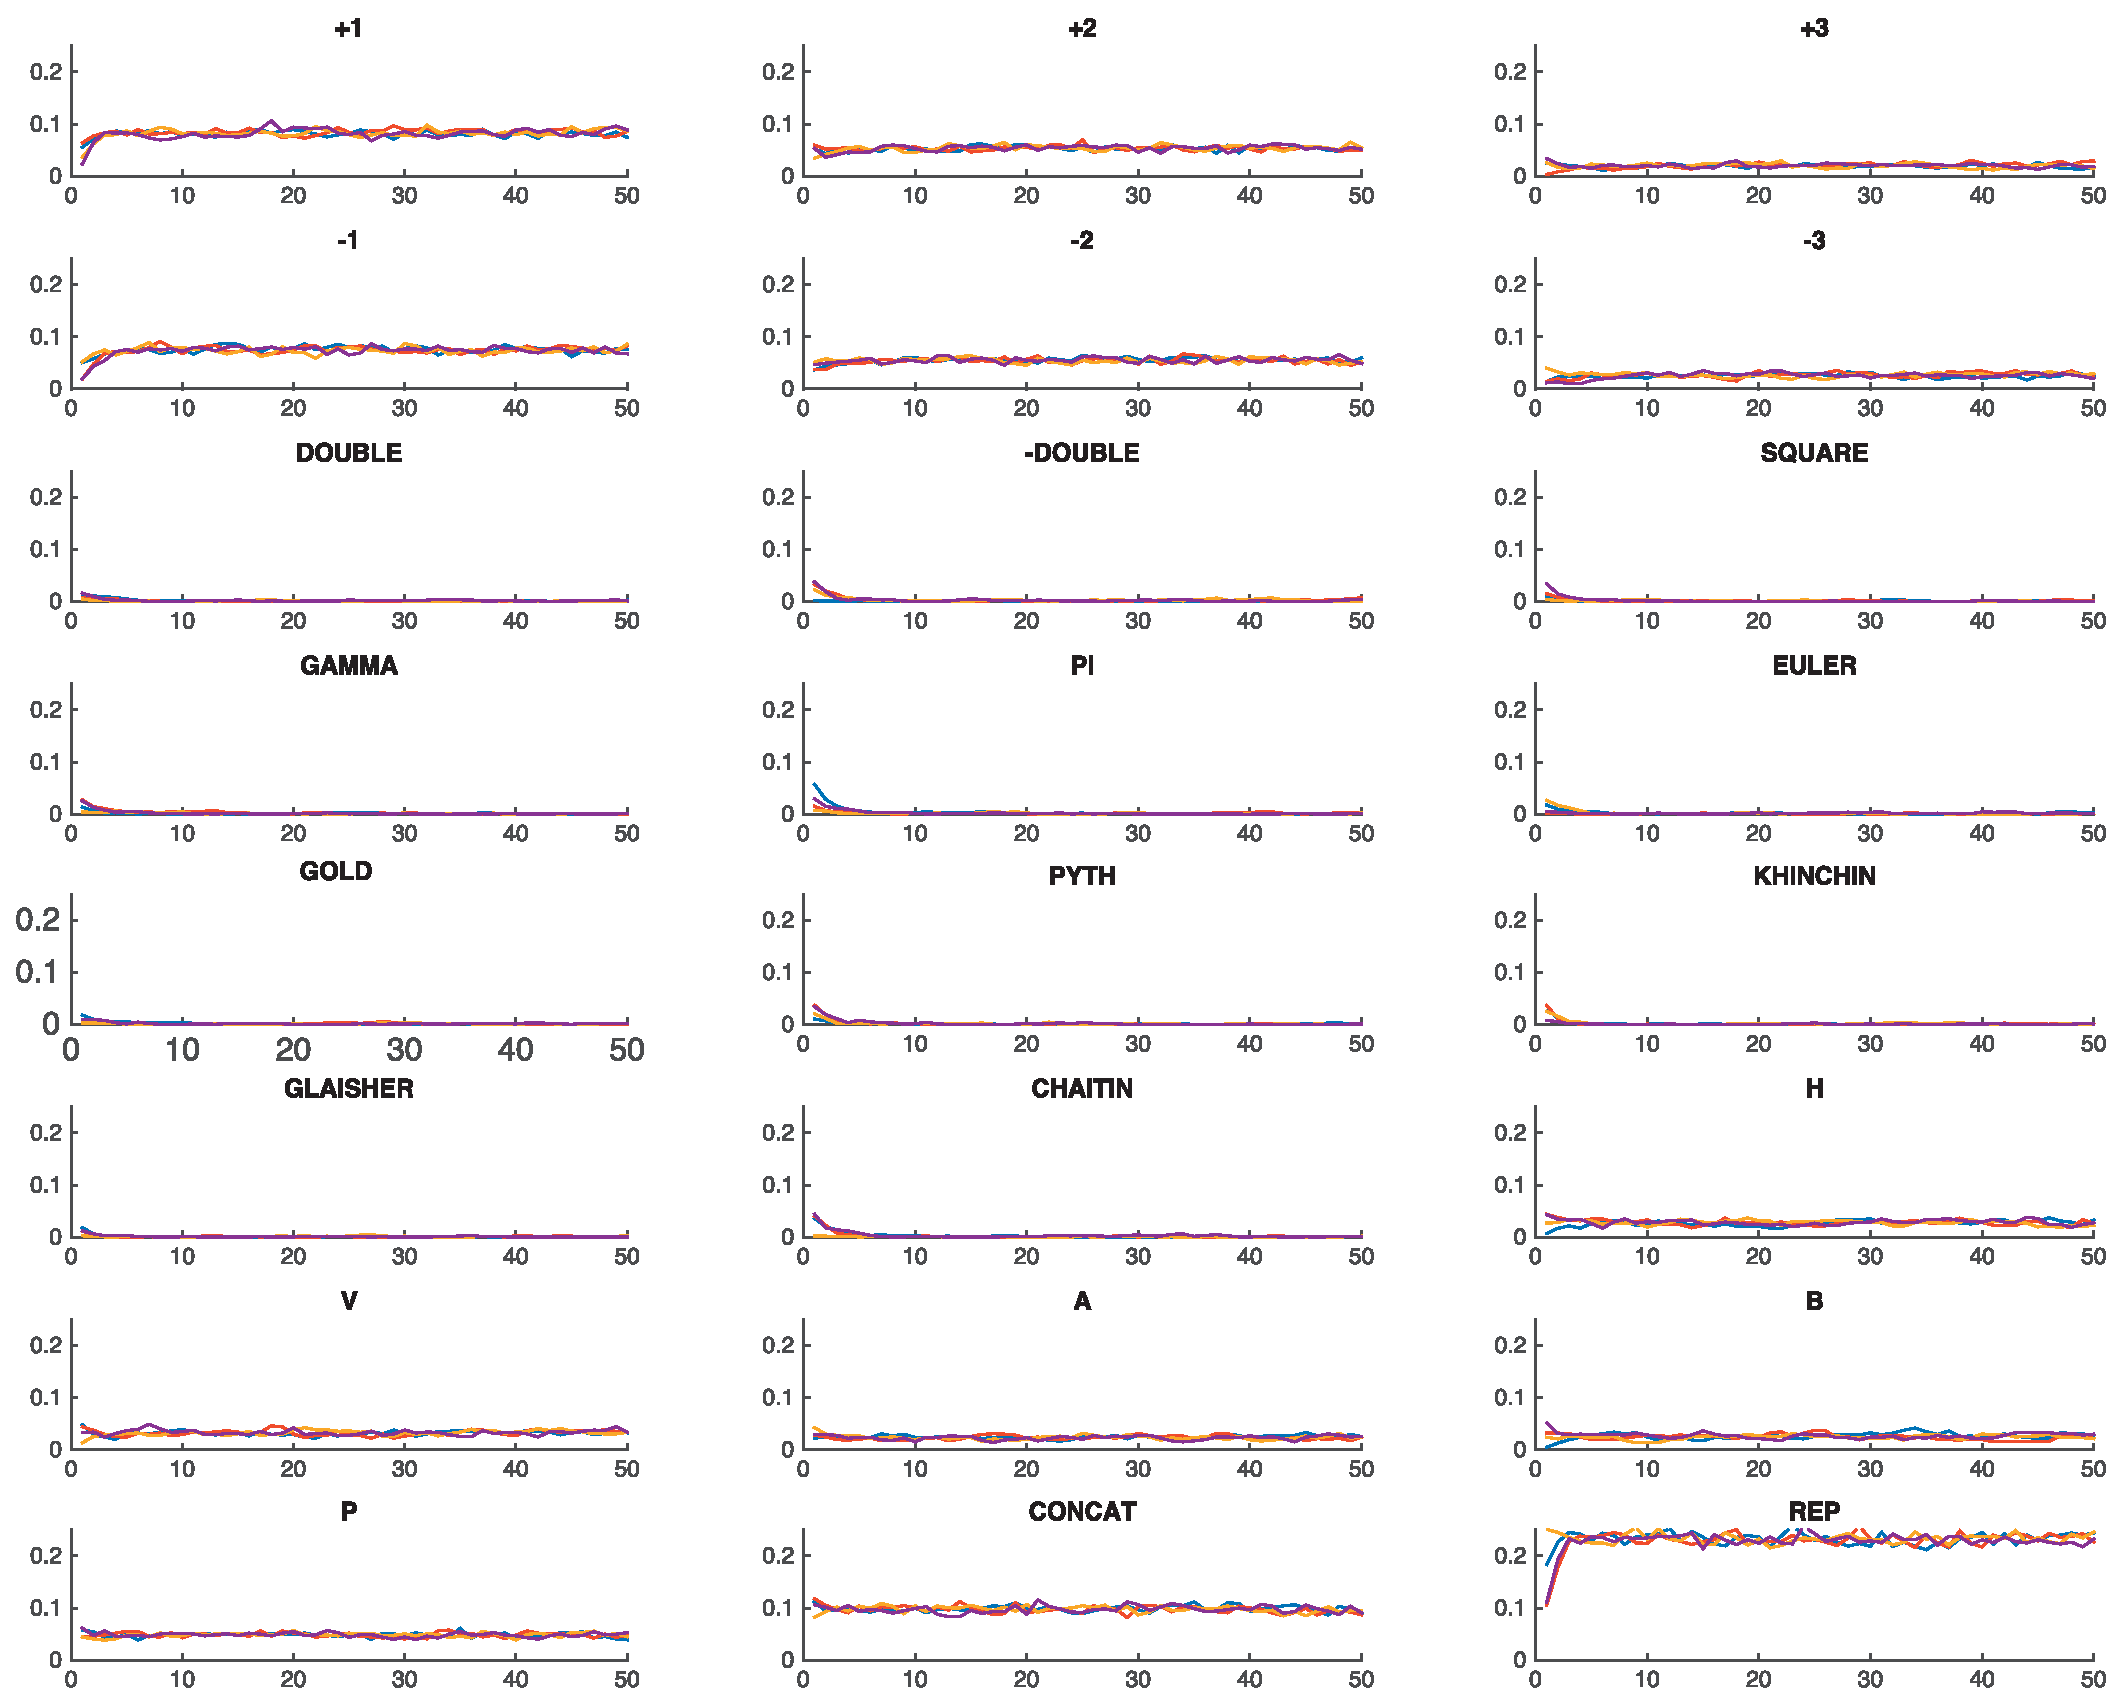
\includegraphics[width=0.8\textwidth]{S1Fig}
    %\caption{\bf{MCMC steps for $\geom$'s productions.} MCMC steps for the rest of $\geom$'s grammar productions.}
    \caption{{\bf Pasos de MCMC para las producciones de $\geom$.} Pasos de MCMC para el resto de las producciones de la gramática $\geom$}
    \label{S1_Fig}
\end{figure}

\begin{figure}[htpb]
    \centering
    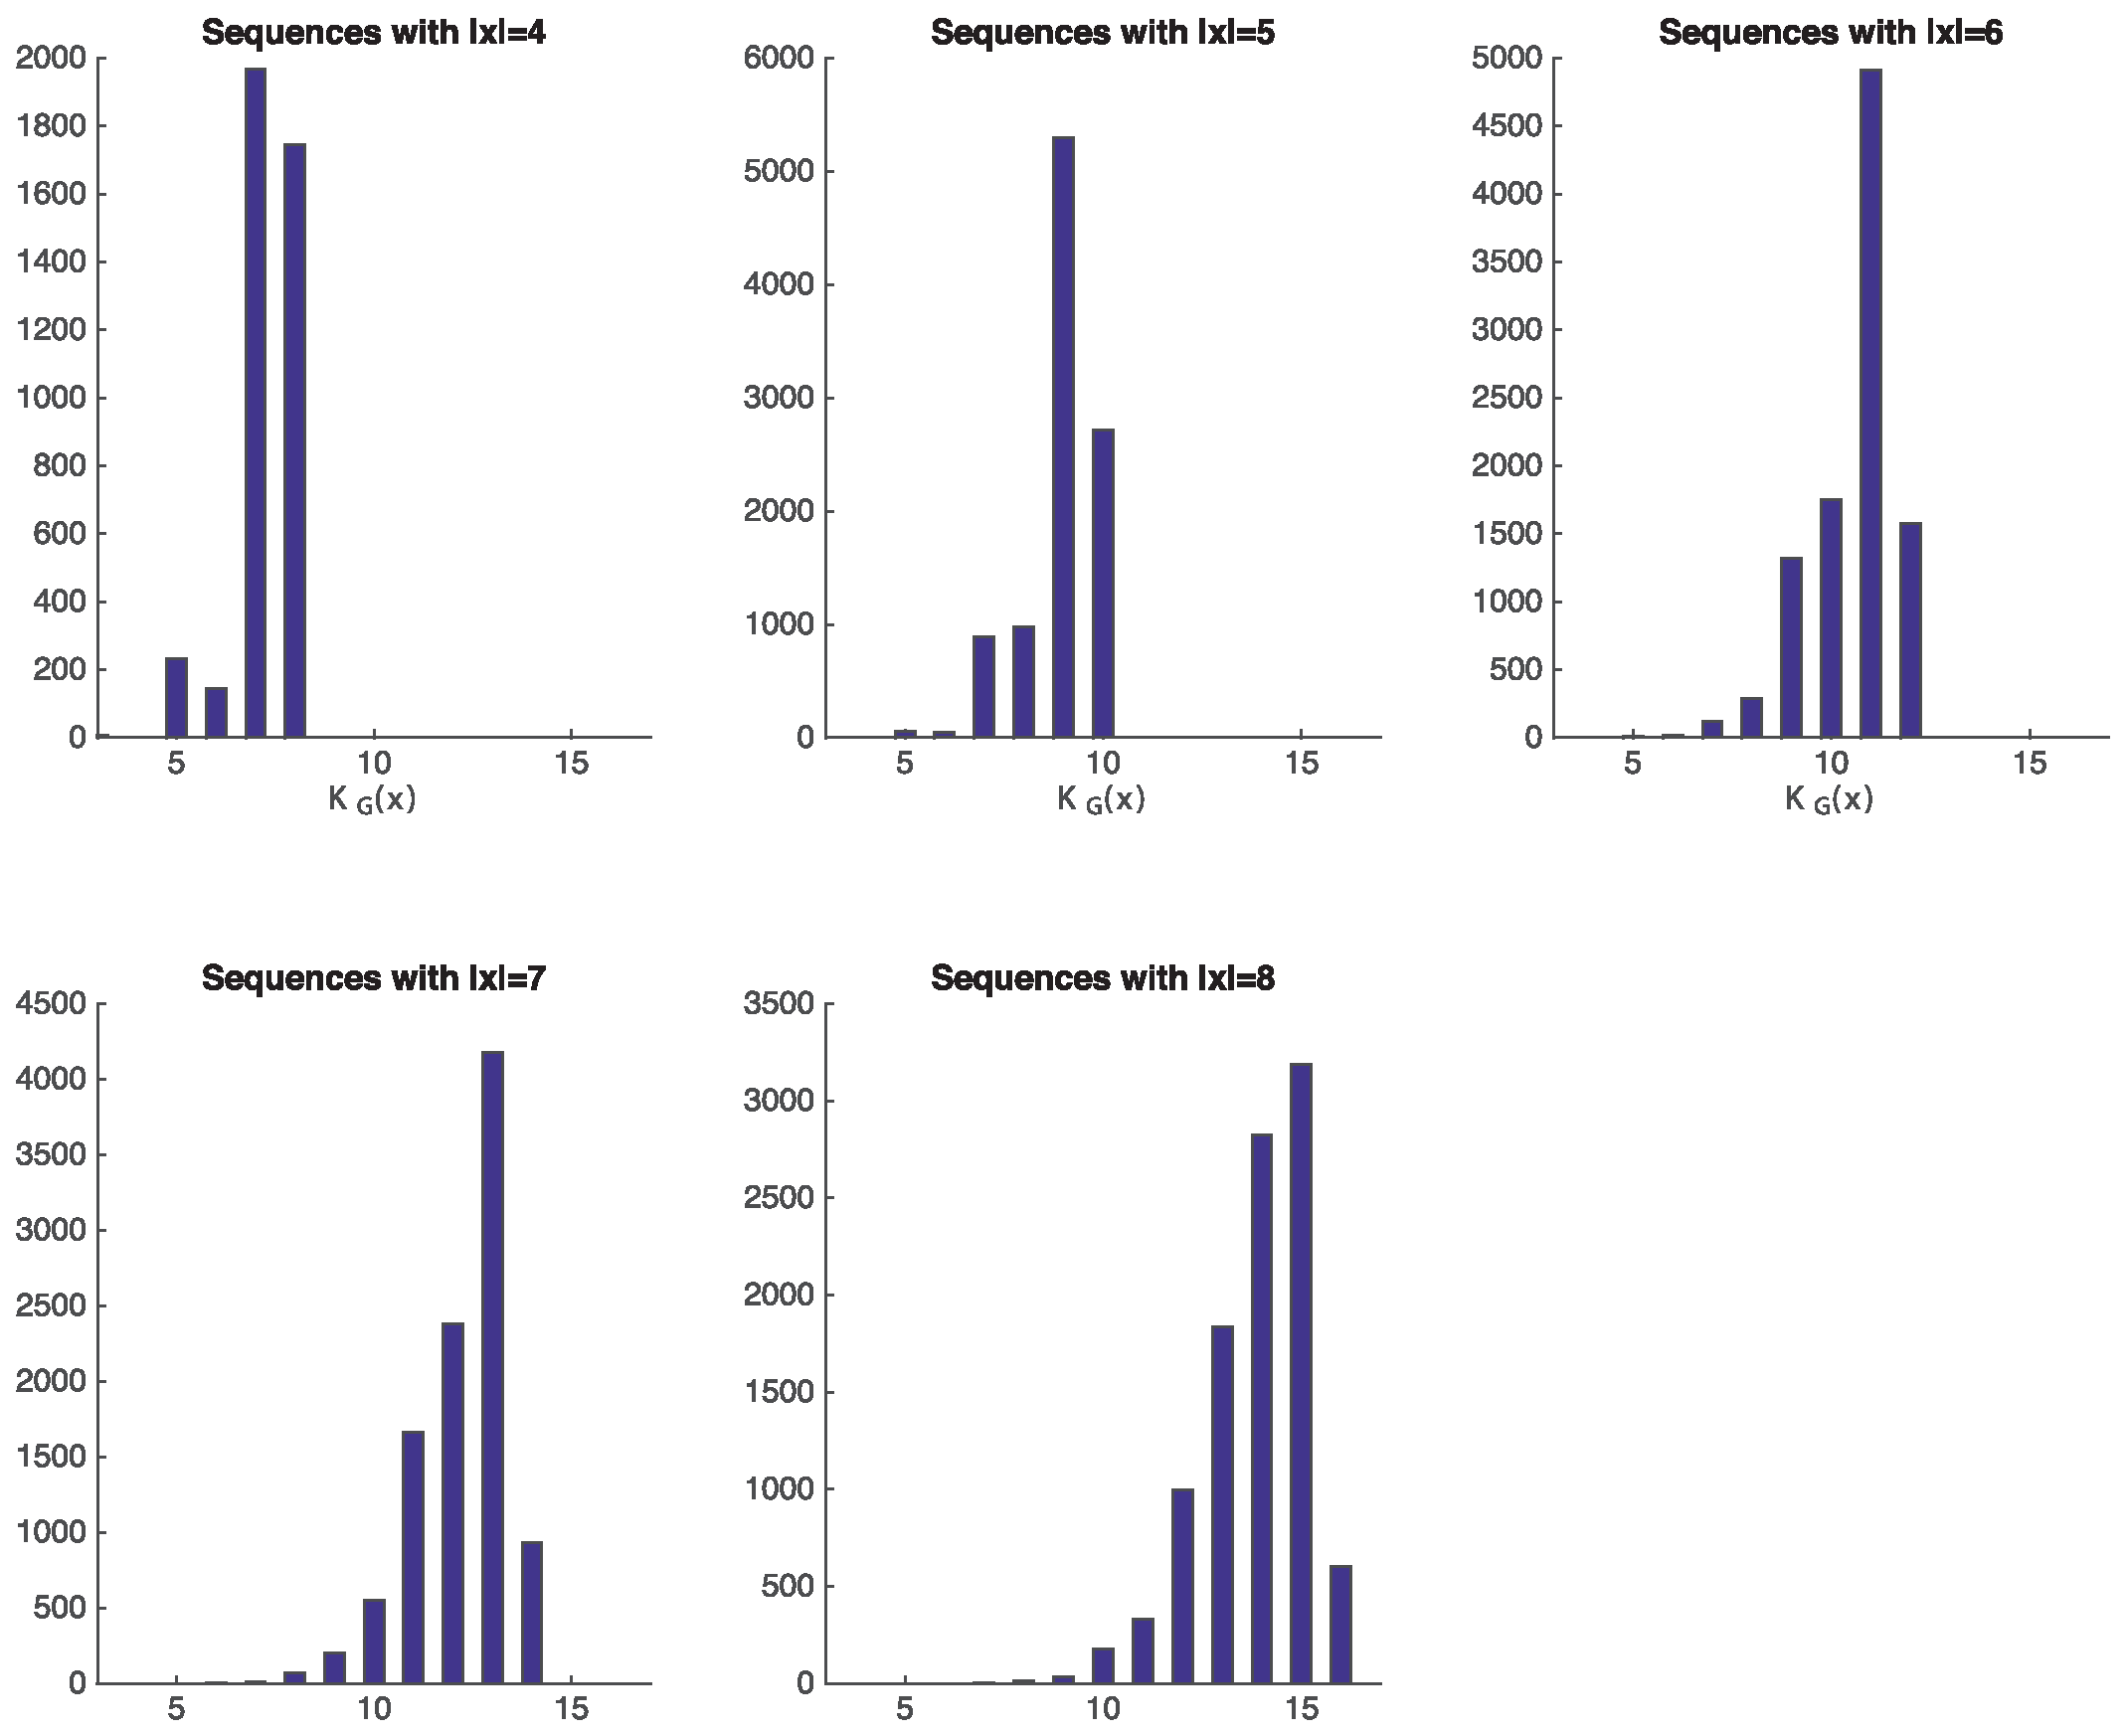
\includegraphics[width=0.8\textwidth]{S2Fig}
    %\caption{\bf{Histograms of complexity $K_{\geom}(x)$}. Histograms of  complexity for sequences with length between 4 and 8.}
    \caption{\bf{Histogramas de complejidad $K_{\geom}(x)$}. Histogramas de complejidad para secuencias con longitud entre 4 y 8.}
    \label{S2_Fig}
\end{figure}

\begin{figure}[htpb]
    \centering
    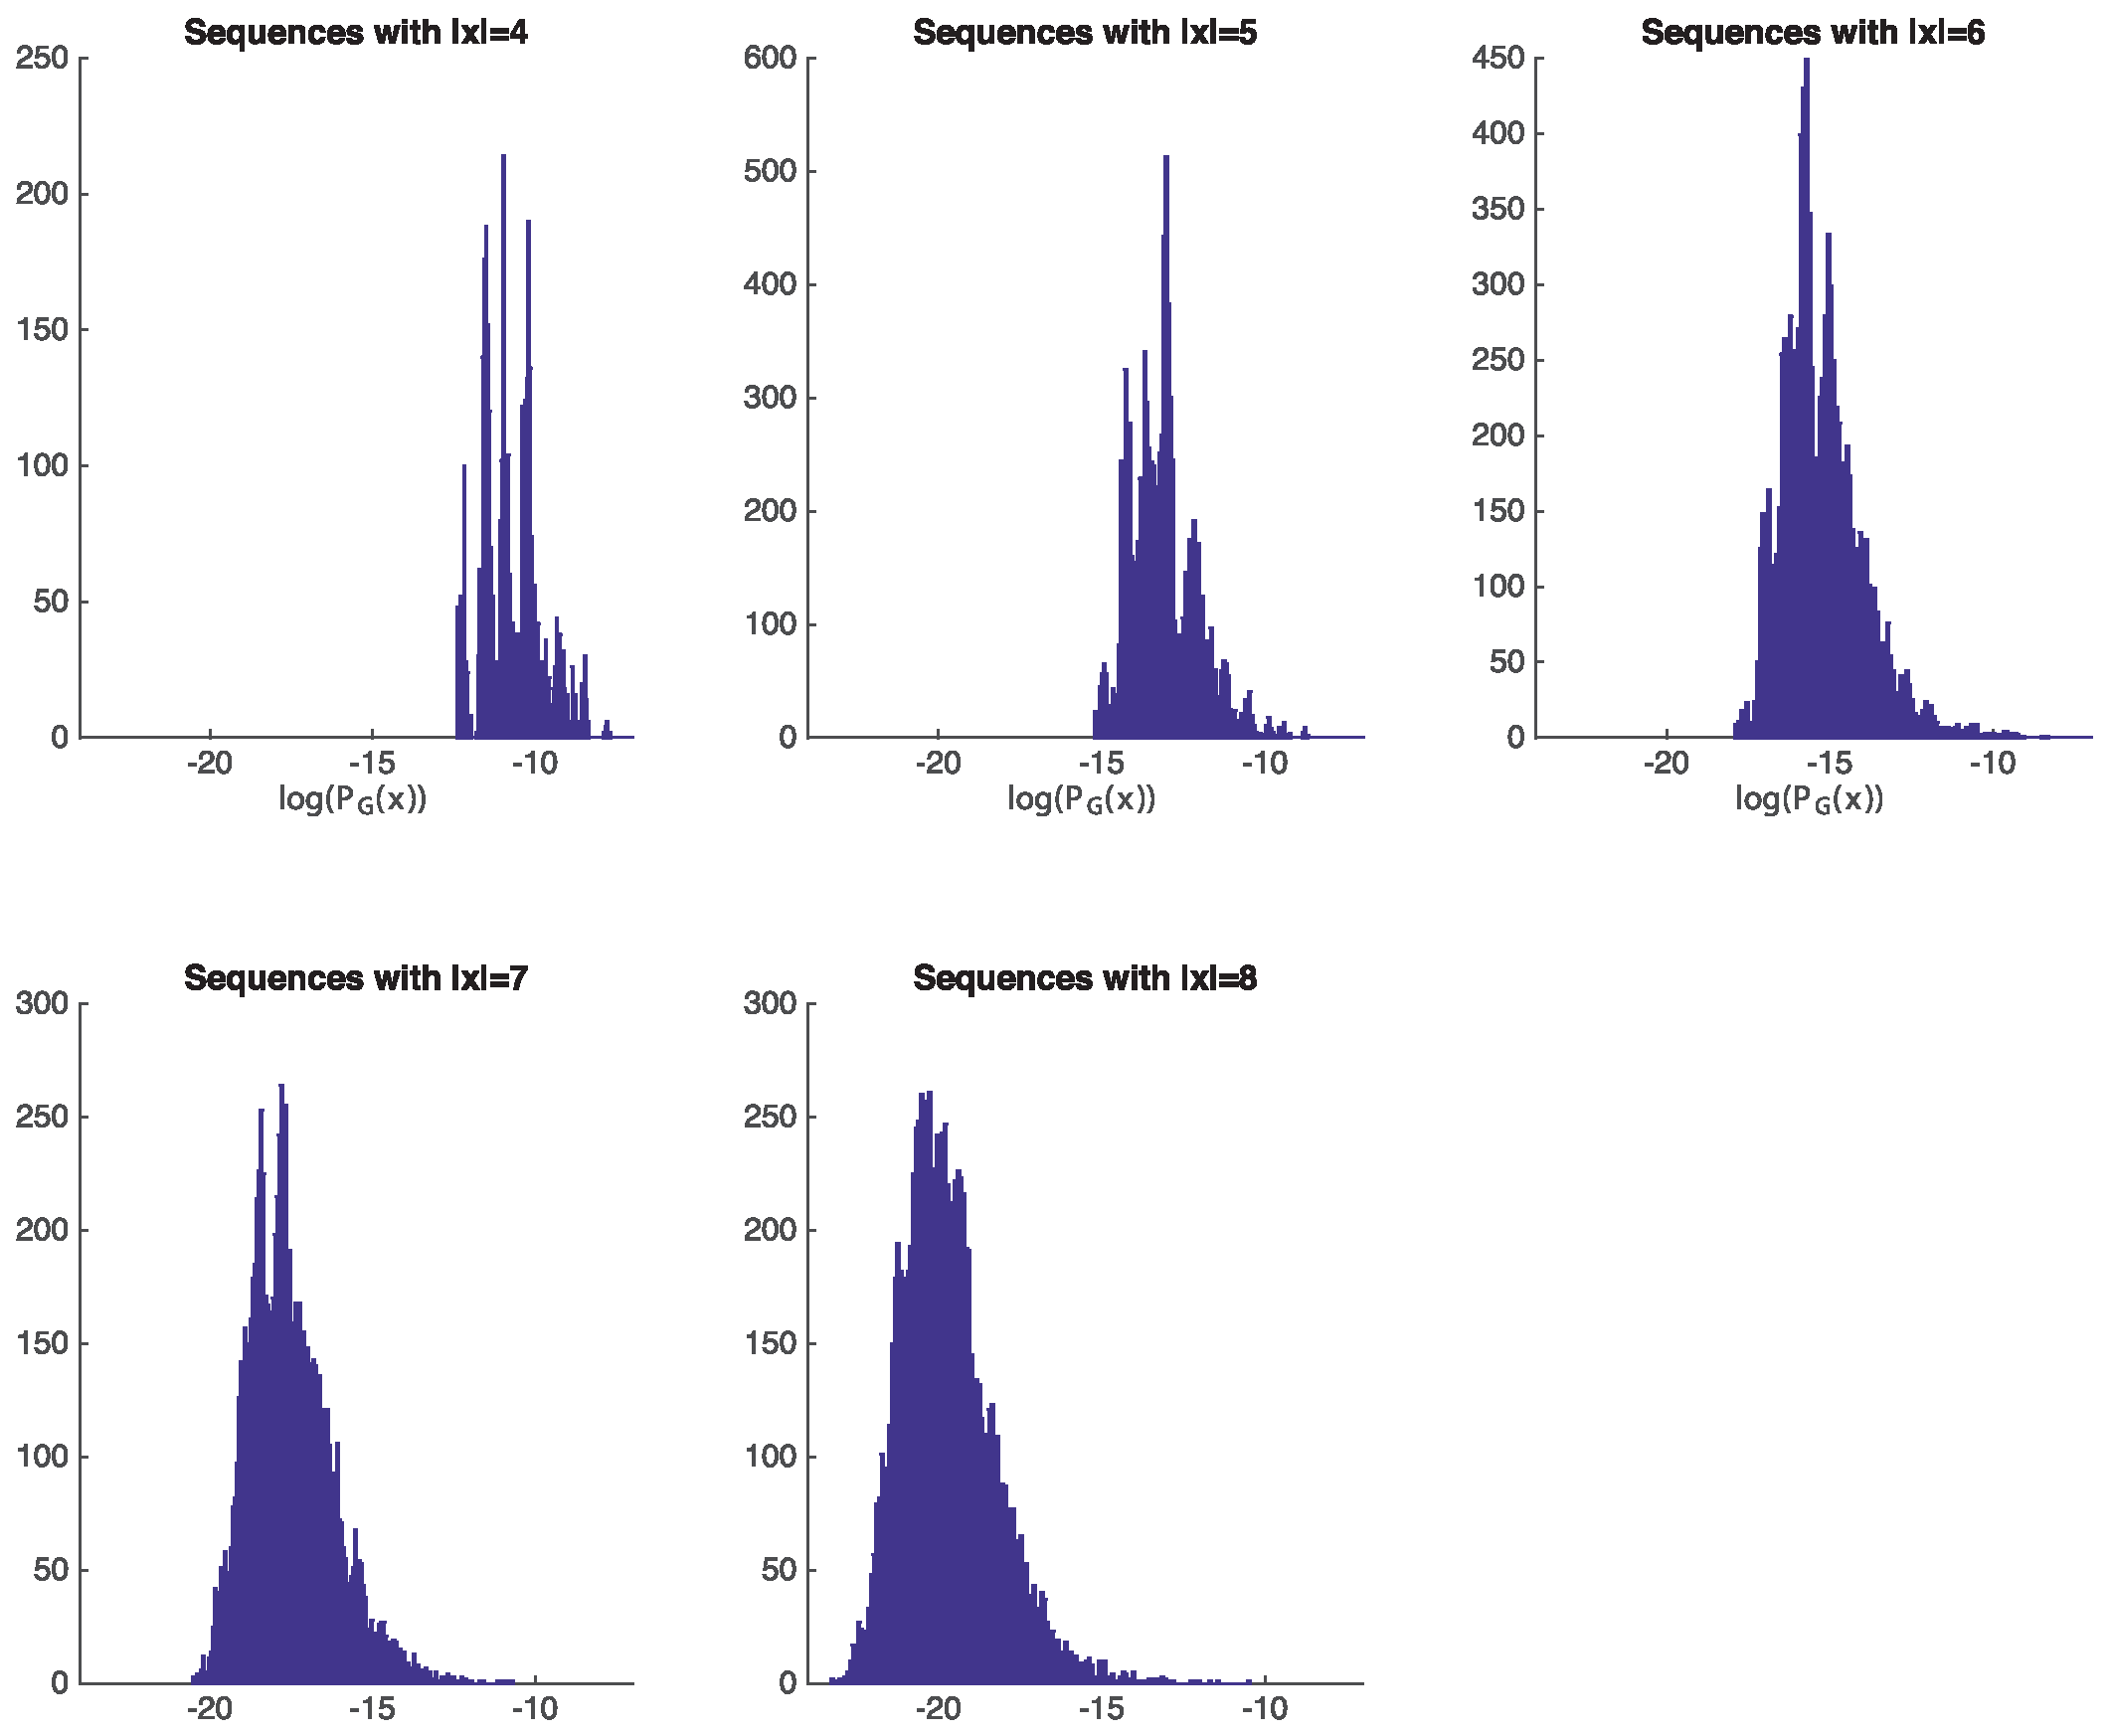
\includegraphics[width=0.8\textwidth]{S3Fig}
    %\caption{\bf{Histograms of probability $P_{\geom}(x)$}. Histograms of  probability for sequences with length between 4 and 8.}
    \caption{\bf{Histogramas de probabilidad $P_{\geom}(x)$}. Histogramas de probabilidad para secuencias con longitud entre 4 y 8.}
    \label{S3_Fig}
\end{figure}